\section{Introduction}
Verification of sequential circuits is challenging, and therefore a topic of continuous research. With
the increasing size of new 
integrated circuits, sequential circuit designers face much more complicated problems of design errors in
specification models and implementations. These errors are usually modeled as ``bad" states,
and the circuits/functional components are modeled as state machines. Once state reachability is analyzed,
the existence of errors can be identified by judging whether ``bad" states are reachable from certain initial states.
Reachability analysis can be performed by various techniques such as extensive simulation, temporal logic model checking
and property directed reachability (PDR). In this proposal we discuss a new promising approach that applies implicitly on the
word level and borrows concepts from commutative algebra and algebraic geometry.

There are several advantages in exploiting word-level verification: on the one hand, a number of circuit designs have 
their datapaths and/or system-level models described  at the word-level, which include many register transfer level 
(RTL) descriptions,
arithmetic components and cryptographic systems. Using word-level information to do verification is convenient 
and beneficial for interpreting the circuit's function. On the other hand, using word-level instead of bit-level
information is one way of ``abstraction". Abstraction is a key technique to reduce the state space of a finite state machine 
when analyzing a sequential circuit. It is usually done by combining sets of states with similar properties.
During state reachability analysis, if we use bit-level variables to  represent the states, 
the representations may become too large to handle (e.g. BDD explosion). However, when a ``bundle" of bit-level variables are represented as only one
word-level variable, the set of reachable states can be represented by a  word-level constraint 
expression. Word-level 
verification techniques are effective in lowering the complexity of state reachability analysis.

Algebraic geometry can provide a symbolic representation of both bit-level (Boolean) variables and 
word-level variables \textit{in one unified framework}. The basic idea is that values of state variables can be represented as solutions to a 
finite set of polynomials. Gr\"obner basis (GB) techniques can be subsequently
applied to transform such polynomial systems into a unique canonical form, thus facilitating verification.
To represent Boolean circuits at word level, polynomial functions over Galois fields provide a {\it bit-precise
word-level model}.
%bit, word ,\Fkk
Particularly, arbitrary word-level datapaths can be modeled as polynomial
functions over $\Fkk$ -- i.e. the Galois field of $2^k$ elements, where $k$ represents the bit-vector word length. In this fashion,
%\footnote{currently no theory can guarantee unique one-to-one mapping for polynomials 
%from $\mathbb B^k$ to $\mathbb Z_{2^k}$ yet}.
%Need introduce \Fkk first
the states and transition relations can be represented as polynomial functions over $\Fkk$ and the power of algebraic geometry can be applied to
implement symbolic reasoning about state reachability. This kind of implicit state
analysis and abstraction can overcome scalability issues encountered by explicit bit-blasting.
Recent work of T. Pruss \cite{timDAC}, J. Lv \cite{jinpeng}, A. Lvov \cite{BLUEVERI} and M. Brickenstein \cite{PolyBoRi}
shows that it is possible to make application of algebraic geometry practical for circuits.

\textbf{This proposal investigates a wide gamut of symbolic computation and algebraic geometry techniques for reachability analysis, abstraction and
verification of sequential circuits applied at the word level.}

%Above example shows how algebraic geometry can be applied to induce one-step reachability. 
% : every function on $k$-bit Boolean vector $f:\mathbb B^k\to \mathbb B^k$ 
% can be uniquely mapped to a polynomial function about $k$-bit word from Galois field $\mathcal F:\Fkk \to \Fkk$,
% this word represents a word-level state variable. Thus, the state space with explicit Boolean bits encoding
% can be uniquely mapped to solution (variety) of a set of polynomials (ideal). Then other concepts from algebraic
% geometry are introduced to solve the reachability problem.

The essence of our approach relies on  bit-level to word-level abstraction.
Any Boolean function over $k$-bit vectors $f:\mathbb B^k\to \mathbb B^k$ 
can be uniquely mapped to a polynomial function over $k$-bit words in the Galois field $f:\Fkk \to \Fkk$ \cite{timDAC}. 
Therefore, the transition relation of sequential circuits can be modeled at word level. The set of
states (Boolean encoding) can be represented as (word-level) elements over Galois fields. Verification
requires operations such as image computations, set intersections, unions and complements, unsatisfiability 
(UNSAT) proofs and analysis, etc. The challenge is to discover efficient algorithmic techniques to perform all such 
operations at the word level. While this challenging task is the topic of this research, we
demonstrate the feasibility of this approach in the example below.

\begin{figure}[hbt]
\centering{
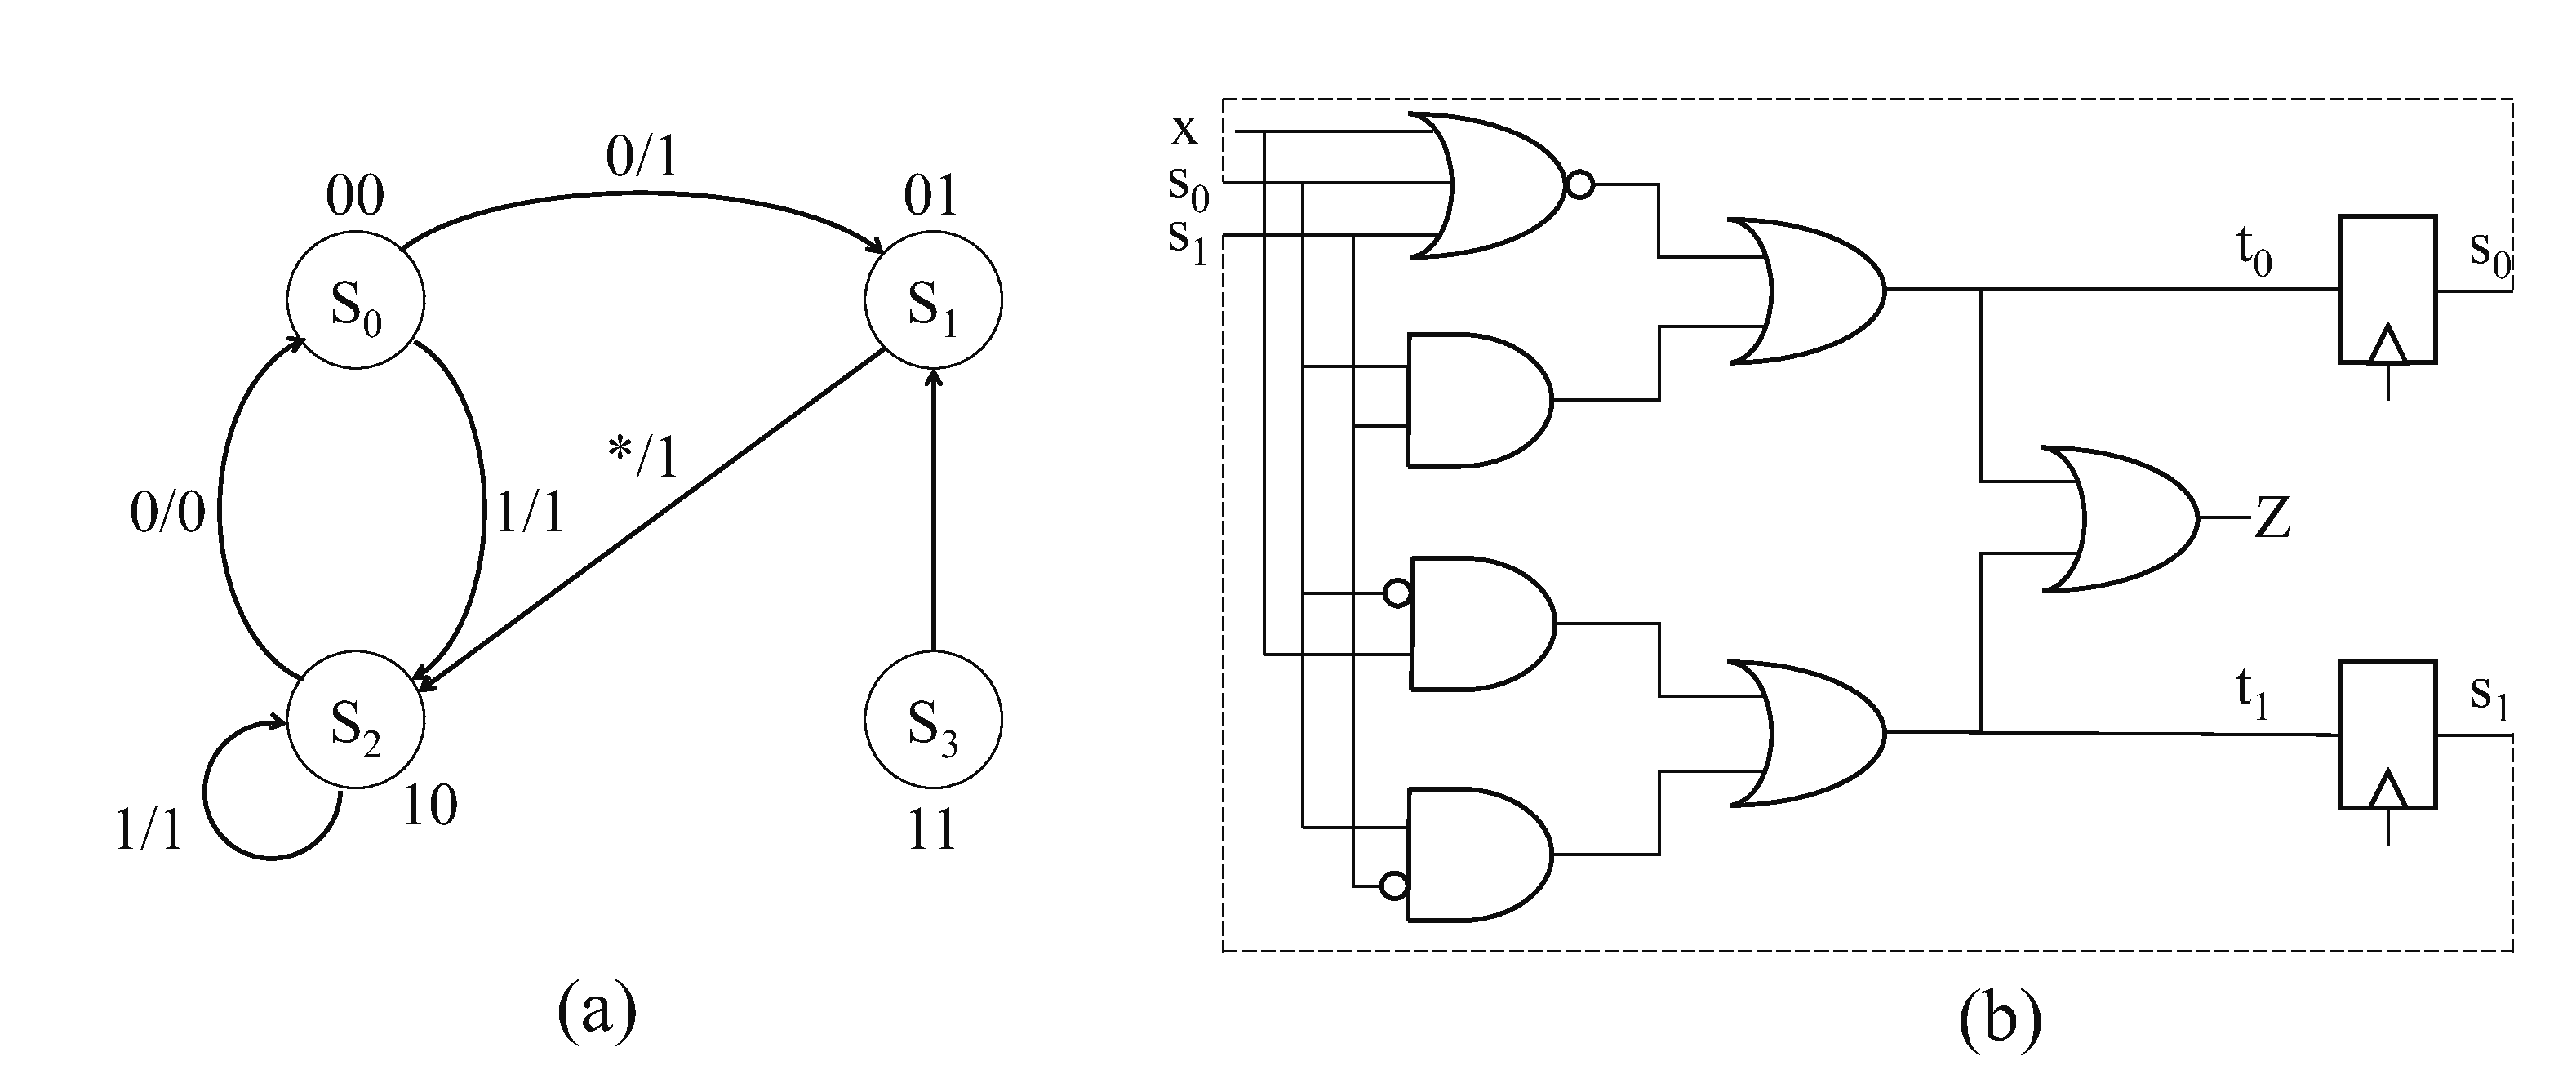
\includegraphics[width=5.5in]{./fig_fsm.eps}
\caption{2-bit FSM example circuit}
\label{fig:fsm}}
\end{figure}

\begin{Example}
\label{ex:motiv}
{\bf Motivating example:} Consider Fig.\ref{fig:fsm}(a), a Mealy finite state machine (FSM) with
4 states encoded by a 2-bit Boolean vector, and Fig.\ref{fig:fsm}(b) as its gate-level circuit implementation.
Variable $x$ is the primary input (PI), $\{s_0,s_1\}$ are present state (PS) variables, $Z$ is primary
output (PO) and $\{t_0, t_1\}$ are next state (NS) variables. The 4 states are encoded as
$\{00,01,10,11\}$, which can be interpreted as elements in $\mathbb F_4$ according to Table \ref{tab:booltof4}.
We can also translate all gates (Boolean operators) to polynomial functions over $\mathbb F_4$.
\vspace{-0.1in}
\begin{table}[htb]
\centering
\caption{Mapping bit-vector state encoding to elements in $\mathbb F_4$, Boolean operators to functions over $\mathbb F_4$}
\begin{tabular}{|c|c||c|c|} 
\hline
Bit-vector & Element in $\mathbb F_4$ & Boolean operator & Function over $\mathbb F_4$ \\
\hline
\hline
00 & 0 & $a\land b$ & $a\cdot b$ \\
\hline
01 & 1 & $a\oplus b$ & $a+b$ \\
\hline
10 & $\alpha$ & $\bar{a}$ & $1+a$ \\
\hline
11 & $1+\alpha$ & $a\lor b$ & $a+b+a\cdot b$\\
\hline
\end{tabular}
\label{tab:booltof4}  
\end{table}

We first obtain polynomials $f_1$ and $f_2$, denoting transition relations for NS $\{t_0,t_1\}$:
\begin{displaymath}
\begin{array}{ll}
f_1:& t_0- (xs_0s_1+xs_0+xs_1+x+s_0+s_1+1) \\
f_2:& t_1 - (xs_0+x+s_0s_1+s_0)\
\end{array}
\end{displaymath}
Since we model reachability at word level, let $S = \{s_0,s_1\}$ represent a word-level PS variable in $\mathbb F_4$,
its relation to bit-level variables is $S = s_0 + s_1\cdot \alpha$, where $\alpha$ is the primitive element
of $\mathbb F_4$. Similarly we can define a word-level NS variable $T$. They can be both interpreted in polynomial form:
\begin{displaymath}
\begin{array}{ll}
f_3:& S - s_0 - s_1\alpha \\
f_4:& T - t_0 - t_1\alpha
\end{array}
\end{displaymath}
The initial state can also be represented in polynomial form. Assume the initial state is $\{00\}$ ($0$ in $\mathbb F_4$),
it corresponds to the solution of the polynomial equation $(S-0) = 0$. So its polynomial form is
\begin{displaymath}
f_5:\  S
\end{displaymath}
We can then use the Gr\"obner basis (GB) computation to compute a canonical form of this system of polynomials
$f_1,\dots, f_5$ representing possible value of NS variable $T$. Note that
if we eliminate the PI variable $x$ from the ideal $\langle f_1,\dots,f_5\rangle$ while computing GB, the result
implies an existential quantification on $x$.

After computing GB with a lexicographic term order $\{x,s_0,s_1,t_0,t_1\} > S > T$, the result contains a polynomial
only in the word-level variable $T$: ${\bf g_T:T^2+(\alpha+1)T+\alpha}$. 
Notice that $g_T$ is a polynomial in word-level variable $T$, it has 2 roots which encode 2 states of the machine  $T = 1(01)\ and 
\ T = \alpha(10)$.
\end{Example}
% \begin{Example}
% \label{ex:motiv}
% {\bf Motivating example:} Fig.\ref{fig:fsm}(a) is a simple 2-bit sequential circuit, it can be modeled
% as a Mealy finite state machine (FSM). $x$ is primary input (one bit),
% $\{s_0, s_1\}$ are state inputs (present state variables), $Z$ is primary output and $\{t_0, t_1\}$ are 
% state outputs (next state variables). Word-level state input (2-bit vector) is $S$, output is $T$.
% Fig.\ref{fig:fsm}(b) shows its state transition graph (STG), states are encoded explicitly with
% present state variables $\{s_0,s_1\}$ taking values from $\{00,01,10,11\}$. Using one-to-one mapping
% $\mathbb B^k \to \Fkk$, we can write word $S$ as element in $\mathbb F_4$: $S = s_0 + s_1\cdot\alpha$, 
% and $T = t_0 + t_1\cdot\alpha$. Here $P(\alpha) = \alpha^2+\alpha+1 = 0$ is the primitive polynomial
% of $\mathbb F_4$.
% 
% We can translate all gates (Boolean operators) to polynomial functions and compose an ideal for this circuit.
% First, transition functions at bit level:
% \begin{displaymath}
% \begin{array}{ll}
% f_1:& t_0- (xs_0^2\cdot s_1^2+xs_0^2\cdot s_1+xs_0\cdot s_1^2+xs_0+xs_1+x+s_0^2s_1^2+s_0^2s_1+s_0s_1^2+s_0s_1+s_0+s_1+1) \\
% f_2:& t_1 - (xs_0^2\cdot s_1+xs_0^2+xs_0\cdot s_1+x+s_0s_1+s0)\
% \end{array}
% \end{displaymath}
% Followed by bits-to-word definitions using polynomial representation of elements in $\mathbb{F}_4$:
% \begin{displaymath}
% \begin{array}{ll}
% f_3:& S - s_0 - s_1\alpha \\
% f_4:& T - t_0 - t_1\alpha
% \end{array}
% \end{displaymath}
% And an polynomial about initial state ($\{00\}$, i.e. $0$ in $\mathbb F_4$):
% \begin{displaymath}
% f_5:\  S
% \end{displaymath}
% And the rests are vanishing polynomials for each variable:
% $f_6: x^2 - x; f_7: t_0^2 - t_0; f_8: t_1^2 - t_1; f_9: S^4 - S; f_{10}: s_0^2 - s_0;
% f_{11}: s_1^2 - s_1; f_{12}: T^4 - T$
% 
% Note that there is no specification on initial primary input $x$, in Gr\"obner basis (GB) approach this means $x$ is smoothed by
% reversely using Shannon's expansion.
% 
% We use elimination term order: $intermediate\ bit$-$level\ signals\ >\ bit$-$level\ primary\ inputs/outputs\ >\ S\ >\ T$, compute Gr\"obner basis for ideal
% $J = \langle f_1, f_2, \dots, f_{12}\rangle $ to compute GB, the result will include one polynomial $f_T$ contains only variable $T$. In this example,
% GB we get is: 
% $g_1:S;
% g_2:T+t_0+t_1\alpha;
% g_3:S+s_0+s_1\alpha;
% g_4:s_1;
% g_5:t_1+T^2+T;
% g_6:x+T^2+T;
% {\bf g_7:T^2+(\alpha+1)T+\alpha}$.
% Note the last polynomial equals to $T^2-(\alpha+1)T+\alpha$ since coefficients of polynomial representation in $\mathbb{F}_{2^2}$ are
% limited within $\mathbb{F}_{2}$, where $x \equiv -x\ (mod\ 2)$ for any element $x$ in the field. 
% Solution to $g_7 = 0$ is $T = 1\ or \ T = \alpha$, which shows that next
% state the machine just reached is $\{S_1(01), S_2(10)\}$.
% \end{Example}


The above example shows how algebraic geometry can be applied to induce one-step reachability at the word level. 
It is possible to combine our approach in this example with other techniques inspired by concepts and theorems
from algebraic geometry to help reachability analysis for FSMs, as well as further formal verification problems
on sequential circuits.

{\bf Contributions of the dissertation:} Our approach to solve the sequential circuit verification problem and contribution
of the thesis can be described as follows:
\begin{itemize}
\item[-] This proposal will investigate techniques to perform sequential circuit verification at the word level
using polynomial abstractions of Boolean circuits over Galois fields. The applications considered are exact
reachability analysis and property directed reachability \cite{bradley2011sat} \cite{bradley2011incremental}. Both sequential datapath circuits
as well as random logic controllers will be considered. 
%%%%%%%%%%%%%%%%%%%%%%%%%%%%%%%%%%
%\item[-] Using polynomial abstractions, we analyze the circuit, and model the gate-level Boolean operators as elements of a
%multivariate polynomial ring with coefficients in $\Fkk$.
\item[-] Algebraic geometry based techniques will be researched for reachability analysis. 
The concepts of Nullstellensatz, Gr\"obner bases and elimination ideals will be explored for 
the purpose of image computations. The canonical representations of polynomial ideals provided
by Gr\"obner bases will be exploited for verification.
%deduce that the one-step reachability problem can be formulated as one of computing a Gr\"obner basis of the set of
%polynomials derived from the given circuit netlist, using a specific elimination term order.
\item[-] Computing Gr\"obner bases for large circuits is infeasible due to its high computational complexity.
Therefore, based on inspirations from \cite{timDAC} and \cite{jinpeng}, a significant part of this work will focus on improving the scalability of our approach.
%\item[-] Apply our approach for one-step reachability to a breath-first search (BFS) state space traversal
%algorithm, the reachability of system can be analyzed when reaching a fixpoint.
%\item[-] Computing Gr\"obner bases using elimination term orders is infeasible for large circuits. 
%To overcome this limitation we introduced improved approach using new term order and variable substitution, 
%as well as F-4 algorithm to accelerate multivariate division.
\item[-] New paradigms for abstraction refinement using algebraic geometry will be explored.
Such techniques require analysis of UNSAT proofs of the verification instances.
UNSAT cores in polynomial calculus have not been researched before. In this proposal,
we will investigate a new technique to identify minimal UNSAT cores using the Gr\"obner basis algorithm 
and apply it to verification.
%and we propose a new
%GB based technique to compute UNSAT core to assist abstraction refinement procedure.
\end{itemize}
%In this proposal, I will show that conceptually our proposed approach is feasible and we will research
%efficient symbolic computing techniques for sequential verification based on algebraic geometry.
All in all, this proposal aims to discover an altogether new paradigm for formal verification/model checking
of sequential circuits at the word level using a combination of design automation, algebraic geometry and 
symbolic computation techniques. Bit-level Gr\"obner basis computation has been applied to model 
checking \cite{avrunin1996symbolic} \cite{tran2007groebner} and satisfiability problems \cite{PolyBoRi},
but Gr\"obner basis at word level has never been explored before for circuit verification.


This proposal is organized as follows: 
Section II reviews preliminary finite state machine and algebraic geometry concepts related to ideals, varieties, Gr\"obner bases, elimination ideals, etc.
Section III describes our proposed approach to perform implicit state enumeration at word level.
An algorithm to extract UNSAT cores based on algebra geometry techniques is conjectured in Section IV. 
Section V outlines the proposed objectives. Finally, Section VI outlines the proposed research timeline.